\documentclass[a4paper,12pt,hidelinks]{report}
\usepackage{array}
\newcolumntype{P}[1]{>{\centering\arraybackslash}p{#1}}
\newcolumntype{M}[1]{>{\centering\arraybackslash}m{#1}}\usepackage[pagebackref=true]{hyperref}
\usepackage{amsmath}
\usepackage{harvard}
\usepackage{mathtools}
\usepackage{graphicx}
\usepackage{float}
\usepackage{subfigure}
\usepackage{epsfig}
\usepackage[inner= 4cm, outer=2cm, top=3cm, bottom=3cm]{geometry}
\usepackage{setspace}
\renewcommand{\baselinestretch}{1.5}
\usepackage{amsfonts}
\usepackage{caption}
\usepackage[font=small,labelfont=bf]{caption}
\usepackage{algorithm}
\usepackage{algpseudocode}
\usepackage{enumerate}
\usepackage{listings}
\usepackage{xcolor}

\definecolor{codegreen}{rgb}{0,0.6,0}
\definecolor{codegray}{rgb}{0.5,0.5,0.5}
\definecolor{codepurple}{rgb}{0.58,0,0.82}
\definecolor{backcolour}{rgb}{0.95,0.95,0.92}

\lstdefinestyle{mystyle}{
    backgroundcolor=\color{backcolour},   
    commentstyle=\color{codegreen},
    keywordstyle=\color{magenta},
    numberstyle=\tiny\color{codegray},
    stringstyle=\color{codepurple},
    basicstyle=\ttfamily\footnotesize,
    breakatwhitespace=false,         
    breaklines=true,                 
    captionpos=b,                    
    keepspaces=true,                 
    numbers=left,                    
    numbersep=5pt,                  
    showspaces=false,                
    showstringspaces=false,
    showtabs=false,                  
    tabsize=2
}

\lstset{style=mystyle}


\setcounter{tocdepth}{3}
\setcounter{secnumdepth}{3}
\begin{document}
\begin{titlepage}
\begin{center}
\begin{huge}
\textbf{*Insert Title Here*}\\
\end{huge}
\vspace{10mm}
\begin{huge}
by \\
PARBHU Varun \\ 
\end{huge}
\begin{large}
\vspace{15mm}
Project Supervisor: Professor (Dr) BHURUTH MUDDUN OSK \\
\vspace{15mm}
Project submitted to the Department of Mathematics,\\
Faculty of Science, University of Mauritius,\\
as a partial fulfillment of the requirement\\
for the degree of\\
\textbf{M.Sc. Mathematical and Scientific Computing (Part time)}\\
\end{large}
\vspace{30mm}
December 2022
\end{center}
\end{titlepage}
\pagenumbering{roman}
\tableofcontents


\listoffigures
\addcontentsline{toc}{section}{\listfigurename}

\listoftables
\addcontentsline{toc}{section}{\listtablename}

\chapter*{Acknowledgement}
\addcontentsline{toc}{section}{Acknowledgement}
First and foremost, I would like to show my deepest gratitude to my supervisor Professor (Dr) M. Bhuruth for his guidance and recommendations throughout the project. Also, I would like to thank my family and friends for their constant support during the coursework.

\noindent Lastly, I would like to thank my colleagues for their constant support.
\chapter*{Abstract}
\addcontentsline{toc}{section}{Abstract}
Cryptocurrencies have been gaining much attention in the past few years due to their steep increase in value. However, they are also more volatile than traditional fiat payment methods backed by a country's government. Moreover, cryptocurrencies are speculative, which fuels the necessity of understanding their behaviour over time. This dissertation studies the principle of deep learning and different sequential neural network architecture. We follow up with a literature review of the state-of-the-art algorithm used to optimise neural networks and sentiment analysis methods. An approach to modelling Bitcoin price over a 24hr period using LSTM NN is proposed. The hourly tweet count, Google search index of the word 'Bitcoin' and sentiment of tweets averaged hourly are input features of the LSTM NN model. During experimentation, the hourly tweet count and the hourly average of tweet sentiment resulted in the lowest training and testing RMSE, \$296.33 and \$189.66, respectively.






% High frequency data have been mushrooming the financial market in recent years. There is a major need to quantify and predict such type of data in a tolerable lapse of time to minimize risk. In this dissertation, the Fast Fourier Transform is studied and implemented into conditional variance models in order to reduce the computa- tion time to estimate the parameters of such models. A study of the convolution sum is performed to determine the calculation advantage the fast Fourier transform ad- vocates over vectorise summation. The fast Fourier transform is implemented in the estimation of parameters of ARCH, GARCH and FIGARCH models, via their log- likelihood function. The speed-up factor was up to 4.0, 11.0 and 5.8 for the ARCH, GARCH and FIGARCH models respectively. A new approach to the problem which consists of a one-time analysis of the algorithm to improve the speed-up factor is pro- posed. We identify that larger sample sizes doesn’t imply greater computation time and smaller sample sizes doesn’t imply lower computation time. Optimal sample lengths are found via experimentation as no theory predicts the latter. By studying the behaviour of the fast Fourier transform algorithm we demonstrate that the new angle to the problem for a FIGARCH model was up to 4 times faster compared to the direct fast Fourier transform implementation. This is a global improvement for the calculation of convolution sum using fast Fourier transform and not just local to financial models.

\nocite{*}
\bibliographystyle{agsm}
\chapter*{Terms and Definitions}
\addcontentsline{toc}{section}{Terms and Definitions}
\begin{tabular}{l | l}
\(\alpha\) & Learning Rate \\
\(\eta\) & Reduced Learning Rate \\
\textbf{I} & Identity Matrix \\
\(\odot\)& Hadamard Product \\
NN & Neural Network \\
LSTM & Long Short-Term Memory \\
MSE & Mean Squared Error \\
MAE & Mean Absolute Error \\
NLP & Natural Language Processing \\
\end{tabular}

\newpage

\pagenumbering{arabic}
\chapter{Introduction}
A cryptocurrency is a decentralised digital asset distributed over an extensive network of computers. Bitcoin was the first cryptocurrency to be operational in January 2009 after the appearance of the mysterious paper titled ”Bitcoin: A Peer-to-Peer Electronic Cash System”, published in 2008 under the alias “Satoshi Nakamoto” (a person or group of people) \cite{satoshi2009}. The paper described a peer-to-peer payment system using electronic currency (cryptocurrencies) that could be sent directly from one party to another without using a third party (often a financial institution) to validate the transaction. The main idea behind the paper was to emulate an online shared ledger on the peer-to-peer network to validate all transactions via a blockchain, eliminating the risk of forging the register. Hence, the rise of blockchain technology provides security, privacy and a distributed ledger applicable in IoT, distributed storage systems and many more. In exchange for maintaining the blockchain (run and validate), which is energy dependent on running electronic machines, “miners” are rewarded with cryptocurrency.

\par The value of such a type of currency is highly volatile and speculative. It is different from any other asset on the financial market and thereby creates new possibilities for stakeholders with regard to risk management, portfolio analysis and consumer sentiment analysis \cite{Anne2016}. Bitcoin had a market cap of over \$ 300B in December 2022. From basically nothing in January 2009 to reaching the highest price (known to date) of \$67,566.83 on November 8, 2021, Bitcoin has been highly volatile compared to other traditional forms of FIAT payment. During that time, there have been substantial price changes over short periods. In 2017 the value of a single Bitcoin increased from \$863 on January 9, 2017, to a high of \$17,550 on December 11, 2017 \cite{Abraham2018}. Due to its volatility and never seen behaviour like traditional currencies, Bitcoin (and cryptocurrencies in general) are extremely difficult to predict. Nevertheless, it was found that the best model for Bitcoin price volatility is the AR-CGARCH model, highlighting the significance of including both a short-run and a long-run component of the conditional variance \cite{Paraskevi2017}. Halvor et al. find that the heterogeneous autoregressive model is suitable for Bitcoin volatility whereby trading volume further improves this volatility model \cite{Halvor2019}.

\par In this modern age, social media platforms allow people to share sentiments on a large scale. Hence, prompting research to study the impact of sentiment on different complex problems. Asur and Huberman attempted to solve the revenue prediction of box-office for movies problem using tweet volume and sentiment \cite{Asur2010}. The same kind of data and polling results were also used by Bermingham \& Smeaton to train a linear regression model to predict election results \cite{smeaton2011}. Zhang et al.leveraged sentiments on Twitter to help predict the movement of stock market indices such as Dow Jones, S\&P500 and NASDAQ \cite{Zhang2011}. It was shown that significant negative emotions and opinions caused Dow to go down the next day, and lower negative emotions caused Dow to go up the next day. Consequently, studies are being conducted to correlate the speculative nature of Bitcoin prices and their sentiments on social media. Banerjee et al. studied the impact of cryptocurrency returns and Covid 19-news. A nonlinear technique of transfer entropy was used to investigate the relationship between the top 30 cryptocurrencies by market capitalisation and COVID-19 news sentiment. Results show that COVID-19 news sentiment influences cryptocurrency returns \cite{Banerjee2022}. Zhang et al. explored the cryptocurrency market's reaction to issuers' Twitter sentiments. It was found that cryptocurrency prices react positively to Twitter sentiments \cite{Zhang2022}. In contrast, the trading volume reacts positively to the absolute value of Twitter sentiments in a timely manner (within a period of 24 h).

\par This project introduces the essential concepts of deep learning, optimisation, and sentiment analysis. We then follow up with an application in the prediction of Bitcoin's price. Chapter 2 introduces the perceptron, its development into feedforward neural networks and a derivation of the backpropagation algorithm. In Chapter 3, we looked at the different optimisation algorithms and the application of the Adam algorithm in backpropagation. Then, in Chapter 3, we reviewed the traditional and modern sentiment analysis techniques. An application for the prediction of Bitcoin price using data from different sources, sentiment analysis and LSTM NN is studied in Chapter 5. Finally, the project concludes by summarising all our results, findings, and potential improvements.









%- Discussion around Cryptocurrency and frequency of changes \\
%- Discussion around Twitter and the API (amount of data) \\
%- Discussion around the advancement Compute processing speed and Deep Learning algorithms
\chapter{Methodology}
\section{Introduction}
Deep learning is a multidisciplinary field ranging from linear algebra, calculus and probability theory. With major advancement made in compute processing power; deep learning is commonly used in the industry now.
\section{Linear Algebra}
We introduce briefly the realm of linear algebra to get a better understanding of more complex concepts in neural networks. The focus is set on mainly the properties useful in deep learning. \\
Linear algebra is the study of linear equations of the form:
\begin{equation}
    x_1a_1 + \dots + x_na_n = b
\end{equation}
or as a linear map defined by the following:
\begin{equation}
    (x_1, \dots, x_n) \mapsto (a_1 x_1 + \dots + a_n x_n) \label{eq:2.11}
\end{equation}
and their representation, manipulation and operation using vectors and matrices within a set of predefined axioms. 
\subsection{Vectors}
A vector is quantity that has both a magnitude and direction. It can be represented by an ordered set of numbers or graphically using an arrow.
Consider the vector \textbf{u} in $\mathbb{R}^2$ given by:
\begin{align}
    \textbf{u} &= \begin{bmatrix}
           u_1 \\
           u_2 \\
         \end{bmatrix}
  \end{align}
The vector can be expressed graphically as shown below.
\begin{center}
    *Image Placeholder vector in $R^2$*    
\end{center}

\noindent The length of the arrow is an indication of the magnitude of a vector and its orientation given by the direction in which the arrow is pointing. The magnitude of the above vector can be computed as such:
\begin{align}
    ||\textbf{u}|| = \sqrt{u_1^2+u_2^2}
\end{align}

\noindent The direction of the vector with respect to the $x$-axis is given by: 
\begin{align}
    \theta = \tan^{-1}\left(\dfrac{u_2}{u_1}\right)
\end{align}
A vector space is a set of vectors which satisfy the following axioms:
\begin{center}
    *Placeholder - Table of Axioms for Vector Space*    
\end{center}
\noindent\textbf{Geometry representation of addition and subtraction of vectors in $\mathbb{R}^2$}
Vector addition and subtraction is performed componentwise along each element of two vectors. Consider the two vectors $\textbf{a}$ and $\textbf{b}$ where:
\begin{align}
    \textbf{u} = \begin{bmatrix}
        u_1 \\
        u_2 \\
      \end{bmatrix},
      \textbf{v} = \begin{bmatrix}
        v_1 \\
        v_2 \\
      \end{bmatrix}
\end{align}
\noindent\textbf{Addition} \\
The addition of vector $\textbf{u}$ and $\textbf{v}$ is given by:
\begin{align}
    \textbf{u} + \textbf{v} =
      \begin{bmatrix}
        u_1 + v_1 \\
        u_2 + v_2 \\
      \end{bmatrix}
      \label{eq:addition_vectors}
\end{align}
The geometrical effect of adding $\textbf{u}$ and $\textbf{v}$ together is shown below.
\begin{center}
    *Image Placeholder vector addition in $R^2$*    
\end{center}
We can observe from (image ref) above that adding $\textbf{u}$ to $\textbf{v}$ has the effect of rotating $\textbf{u}$ towards $\textbf{v}$.

\noindent\textbf{Subtraction} \\
The subtraction of vector $\textbf{v}$ from $\textbf{u}$ is given by:
\begin{align}
    \textbf{u} - \textbf{v} =
      \begin{bmatrix}
        u_1 - v_1 \\
        u_2 - v_2 \\
      \end{bmatrix}
      \label{eq:subtraction_vectors}
\end{align}
\begin{center}
    *Image Placeholder vector subtraction in $R^2$*    
\end{center}
We can observe from (image ref) above that subtracting $\textbf{v}$ from $\textbf{u}$ has the effect of rotating $\textbf{u}$ in the opposite direction of $\textbf{v}$.\\
\vspace{1mm}
\noindent The effect of rotating two vectors though addition and subtraction are useful properties utilized in deep learning.
\subsubsection{Inner Product}
\noindent The inner product or dot product of: 
\begin{align}
    \textbf{u} = \begin{bmatrix}
        u_1 \\
        u_2 \\
      \end{bmatrix},
      \textbf{v} = \begin{bmatrix}
        v_1 \\
        v_2 \\
      \end{bmatrix}
\end{align}
is given by $\textbf{u}.\textbf{v}$
\begin{align}
  \textbf{u.v} &= u_1 v_1 + u_2 v_2 \\
  &= ||\textbf{u}|| \, ||\textbf{v}||\cos \theta
  \label{eq:cosine_rule_dot_product}
\end{align}
where $\theta$ is the angle between vectors \textbf{u} and \textbf{v}.
\begin{center}
  *Image Placeholder inner product in $R^2$*    
\end{center}
The dot product of $\textbf{u.v}$ equals \textbf{v.u}. The order does not make a difference.
\subsection{Matrices}
\noindent A matrix is an $m \times n$ array of numbers, where $m$ is the number of rows and $n$ is the number of columns; the matrix is said to be of dimension $(m \times n)$.
\begin{align}
  \textbf{A} = 
  \begin{bmatrix}
    a_{11} & a_{12} & \dots & a_{1n} \\
    a_{21} & a_{22} & \dots & a_{2n} \\
    \vdots & \vdots & \ddots & \vdots \\
    a_{m1} & a_{m_2} & \dots & a_{mn}
  \end{bmatrix}
\end{align}
Similar to vectors, there are a couple of matrix operations that can be done under certain condition. \\
\noindent \textbf{Matrix Operations} \\ 
\noindent \textbf{Matrix Addition} \\
The sum of two matrices $\textbf{A}$ and $\textbf{B}$ is given by the element wise sum of the elements provided that they both have the same dimension. 
\\ Consider two matrices \textbf{A} and \textbf{B}:
\begin{align}
  \textbf{A} =
  \begin{bmatrix}
    a_{11} & a_{12} \\
    a_{21} & a_{22}
  \end{bmatrix} \, \, \, 
  \textbf{B} =
  \begin{bmatrix}
    b_{11} & b_{12} \\
    b_{21} & b_{22}
  \end{bmatrix}
\end{align}
 the sum \textbf{A + B} is given by
\begin{align}
  \textbf{A} + \textbf{B} = \begin{bmatrix}
    a_{11} + b_{11} & a_{12} + b_{12} \\
    a_{21} + b_{21} & a_{22} + b_{22}
  \end{bmatrix}
\end{align}\\
\noindent \textbf{Scalar Matrix Multiplication} \\
The product $\alpha\textbf{A}$, where $\alpha \in \mathbb{R}$ and $\textbf{A}$ is a matrix, is calculated by multiplying every entry of $\textbf{A}$ by $\alpha$. \\
Consider  a matrix \textbf{A} and constant $\alpha$:
\begin{align}
  \begin{bmatrix}
    a_{11} & a_{12} \\
    a_{21} & a_{22}
  \end{bmatrix}
\end{align}
the scalar multiplication $\alpha \textbf{A}$ is given by
\begin{align}
  \alpha \textbf{A} = 
  \alpha \begin{bmatrix}
    a_{11} & a_{12} \\
    a_{21} & a_{22}
  \end{bmatrix}
  = \begin{bmatrix}
    \alpha a_{11} & \alpha a_{12} \\
    \alpha a_{21} & \alpha a_{22}
  \end{bmatrix}
\end{align} \\
\noindent \textbf{Matrix Transpose} \\
\noindent The transpose of a $(m \times n)$ matrix $\textbf{A}$ is calculated by swapping the rows into columns or the columns into rows. This operation result in a $(n \times m)$ denoted as $\textbf{A}^T$. \\
Consider  a matrix \textbf{A}, the transpose is given by $\textbf{A}^T$:
\begin{align}
  \textbf{A} = \begin{bmatrix}
    a_{11} & a_{12} \\
    a_{21} & a_{22}
  \end{bmatrix} \, \, \, 
  \textbf{A}^T = \begin{bmatrix}
    a_{11} & a_{21} \\
    a_{12} & a_{22}
  \end{bmatrix}
\end{align}
\noindent \textbf{Matrix Multiplication} \\
The multiplication operation between two matrices is only defined is the number of columns of the left matrix is the same as the number of rows in the right matrix. If \textbf{A} is a $(m \times n)$ matrix and \textbf{B} is a $(n \times p)$ matrix, then their product \textbf{AB} is the $(m \times n)$ matrix whose entries are given by inner product of the corresponding row of \textbf{A} and the corresponding column of \textbf{B}.\\
Consider two matrices \textbf{A} and \textbf{B}:
\begin{align}
  \textbf{A} =
  \begin{bmatrix}
    a_{11} & a_{12} & a_{13} \\
    a_{21} & a_{22} & a_{23}
  \end{bmatrix} \, \, \, 
  \textbf{B} =
  \begin{bmatrix}
    b_{11} & b_{12} \\
    b_{21} & b_{22} \\
    b_{31} & b_{32}
  \end{bmatrix}
\end{align}
 the matrix multiplication is given by \textbf{AB}
\begin{align}
  \textbf{A}\textbf{B} &= \begin{bmatrix}
    a_{11} & a_{12} & a_{13} \\
    a_{21} & a_{22} & a_{23}
  \end{bmatrix} \begin{bmatrix}
    b_{11} & b_{12} \\
    b_{21} & b_{22} \\
    b_{31} & b_{32}
  \end{bmatrix} \\
  &= \begin{bmatrix}
    a_{11}b_{11} + a_{12}b_{21} + a_{13}b_{31} &  a_{11}b_{12} + a_{12}b_{22} + a_{13}b_{32} \\
    a_{21}b_{11} + a_{22}b_{21} + a_{23}b_{31} &  a_{21}b_{12} + a_{22}b_{22} + a_{23}b_{32}
  \end{bmatrix}
\end{align}
\subsubsection{Outer Product}
\noindent The outer product of two vectors $\textbf{u}$ and $\textbf{v}$: 
\begin{align}
    \textbf{u} = \begin{bmatrix}
        u_1 \\
        u_2 \\
      \end{bmatrix} \, \, \, 
      \textbf{v} = \begin{bmatrix}
        v_1 \\
        v_2 \\
      \end{bmatrix}
\end{align}
is given by $\textbf{u}\otimes\textbf{v}$
\begin{align}
  \textbf{u}\otimes\textbf{v} = \begin{bmatrix}
    u_1v_1 & u_1v_2 \\
    u_2v_1 & u_2v_2
  \end{bmatrix}
\end{align}
The outer product of $\textbf{u}\otimes\textbf{v}$ is not equal to $\textbf{v}\otimes\textbf{u}$; the order does matter. However, the transpose of latter outer product are the same:
\begin{align}
  \textbf{u}\otimes\textbf{v} = (\textbf{v}\otimes\textbf{u})^T
\end{align}
\section{Differential calculus}
Differential calculus is the study of the definition, properties, and applications the derivative of a function. The process of finding the derivative is called differentiation. It is the also referred to as the study of rate of change and slopes of curves. In optimization and deep learning, major concepts of differential calculus are used.
\subsection{Derivatives}
Derivatives are important concept for understanding deep learning. The derivative of a function at a particular point is the rate of change of the output of the function with respect to the input at that point. It is also an indication of the slope of the function at a particular point.\\
The mathematical definition of the derivative of a function $f = f(x)$ at a point $a$ is given by
\begin{align}
  f^{'}(a) &= \frac{df}{d x}(a) \\ 
  &= \lim_{\Delta \rightarrow 0} \frac{f(a+\Delta) - f(a-\Delta)}{2 \times \Delta}
\end{align}
\begin{center}
  *Image Placeholder derivative of a function $f$ at $a$ in $\mathbb{R}^2$  and $\mathbb{R}^3$*    
\end{center}
Since the derivative of a function is an indication of the slope of a function; we can deduce that a minimum or maximum point exists when the derivative is equal to $0$ (may also be indication of an inflection point).

\vspace{5mm}
\noindent \textbf{Derivative of Multivariate Functions}
\subsection{Directional Derivatives}
\subsection{Chain Rule}
 The chain rule is a concept in calculus to help us understand and calculate the derivative for composite functions which can be made up of two or more functions chained together. \\
Suppose that we have two function $f(x)$ and $g(x)$ which are both differentiable and define the composite function $h(x) = f(g(x))$ then the derivative of $h^{'}(x)$ is given by
\begin{align}
  h^{'}(x) &= \dfrac{dh}{dx} \\
  &= f^{'}(g(x))g^{'}(x)
\end{align}
Consider that we  have $y=f(u)$ and $u=g(x)$, a different definition of the composite function $y=f(g(x))$, then the derivative of $y$ is,
\begin{align}
  h^{'}(x)  &= \dfrac{dh}{dx} \\
  &= \dfrac{dh}{du} \dfrac{du}{dx}
\end{align}
\subsection{Hessian}
\section{Optimization}
The optimization problem is a computational problem in which the objective is to find the best of all possible solutions. Deep neural networks is a form of an optimization problem to find the best possible set of weights in order to reduce the error in a network.

\noindent A generic form of an optimization problem is given by 
\begin{align}
  \begin{matrix}
    \nonumber
    \underset{x}{\text{minimize/maximize}} &f(x) & \\
    \text{subject to} &g_i(x) \leq 0, \, \, & i=1,\dots,m \\
    &h_j(x) = 0, & j=1,\dots,p
  \end{matrix}
\end{align} 
\noindent where \\
\indent $f: \mathbb{R}^n \rightarrow \mathbb{R}$ is the objective/loss function to be minimized,\\
\indent $g_i(x) \leq 0$ are called inequality constraints,\\
\indent $h_j(x) = 0$ are called equality constraints, and \\
\indent $m\geq0$ and $p\geq0$

\vspace{5mm}
\noindent If $m=p=0$, the problem is an unconstrained optimization problem.
\subsection{Optimization algorithms}
The solutions to the optimization problem are vital in modern machine learning and artificial intelligence algorithms, which includes weight optimization in deep learning. There are a number of popular optimization algorithm currently developed to solve the problem. Hence, choosing the right algorithm can be challenging as well.
\vspace{5mm}
\noindent We explore few of the gradient-based solution to the optimization below. Gradient-based methods are iterative methods that use the gradient information of the objective function during iterations.

\vspace{5mm}
\noindent\textbf{Newton's Method}\\
For minimizing $f(x)$, $x \in \mathbb{R}$, we need to solve $g(x) = f^{'}(x)=0$. Newton's iteration is given by 
\begin{align}
  x_{n+1} &= x_{n} - \dfrac{g(x_{}n)}{g^{'}(x_n)} \\
          &= x_{n} - \dfrac{f^{'}(x_{}n)}{f^{''}(x_n)}
\end{align}
For multivariate functions we need to minimize $f(\mathbf{x})$ over $\mathbf{x} \in \mathbb{R}^n$, that it
\begin{align}
  \begin{matrix}
    \underset{\mathbf{x}\in\mathbb{R}^n}{min} f(\mathbf{x}), & \,\,\, \mathbf{x} =(x_1,x_2,\dots,x_n)^T \in \mathbb{R}^n
  \end{matrix} 
\end{align}
The Newton's iteration for multivariate function is given by
\begin{align}
  \mathbf{x_{n+1}} = \mathbf{x_{n}} - H(\mathbf{x_n})^{-1}\nabla f(\mathbf{x_n})
\end{align}
where\\
\indent $H(\mathbf{x_n})$ is the Hessian matrix of $f(\mathbf{x})$\\
\noindent We can observe from (equation ref) that calculating the inverse of the Hessian matrix can be computationally very expensive for higher dimensions. Replacing $H(\mathbf{x_n})^{-1}$ by $\alpha \mathcal{I}$ where $\mathcal{I}$ is the identity matrix; we get the \textbf{method of steepest descent} given by
\begin{align}
  \mathbf{x_{n+1}} = \mathbf{x_{n}} - \alpha \textbf{I} \nabla f(\mathbf{x_n})
\end{align}
where $\alpha \in (0,1)$ 
\section{Deep Learning}
%\noindent - Short dive into deep learning and its advancement in recent years
%\noindent - Explanation of OR and XOR functions
Deep learning is part of Machine Learning which deals mainly with computers that can learn either on their own or supervised. The latter can solve problem in the industry ranging from computer vision (image), natural language processing (text), automatic speech recognition (audio), time-series prediction amongst others. Deep learning primarily uses the concept of artificial neural networks, which derivatives from how the human brain works, to solve complex linear and non-linear problem.\\
\indent We start by introducing how a simple perceptron works, and gradually increase the complexity of the network until we reach a deep neural network that can solve non-linear problems.
\subsection{Perceptron}
%- Explanation on neuron and short numeric exercise \\ 
%- Solving the XOR OR function using Perceptron
A perceptron is an analogy to the human neuron. It is a computational model that takes an input (scalar or vector) and learns to classify the latter between two classes (binary classifier). It consists of an input, a weighed sum and an activation function. \\ The mathematical definition a perceptron that maps its input $\textbf{x}$ to an output value $f(\textbf{x})$ using a step function as activation function is given by
\begin{align}
  f(\textbf{x}) =
  \begin{cases}
    1 & \text{if } \textbf{w.x} + b > 0 \\
    0 & \text{otherwise}
    \label{eq:perceptron_def}
  \end{cases}
\end{align}
\begin{figure}[h]
  \centering
  \includegraphics[scale=0.15]{CHAPTER_2/c2_fig_perceptron.jpeg}
  \caption{Perceptron graphical representation}
  \label{fig:perceptron}
\end{figure}\\
From the perceptron mathematical definition \refeq{eq:perceptron_def}, we can observe that the dot product is dependent on the angle between the weight vector (\textbf{w}) and the input vector (\textbf{x}). Using dot product (\refeq{eq:cosine_rule_dot_product}), addition (\refeq{eq:addition_vectors}) and subtraction (\refeq{eq:subtraction_vectors}) of vector property; we can define a learning rule for modifying the perceptron to learn how to classify a set of input.
\subsubsection{Perceptron Learning Rule}
\noindent Consider the two sets of point \textbf{A} and \textbf{B} 
\begin{align}
  \textbf{A} =
  \begin{Bmatrix}
    \begin{bmatrix}
      1 \\ 
      2
    \end{bmatrix}
  \end{Bmatrix}
   \, \, \, 
  \textbf{B} =
\begin{Bmatrix}
  \begin{bmatrix}
    -1 \\
    2
  \end{bmatrix},
  \begin{bmatrix}
    0 \\
    -1
  \end{bmatrix}
  \end{Bmatrix}
\end{align}
and fitting the perceptron function (\refeq{eq:perceptron_def}) to learn how to classify points in each respective set. Let set \textbf{A} and \textbf{B} be class 1 and 0 respectively.
\begin{figure}[h]
  \centering
  \includegraphics[scale=0.15]{CHAPTER_2/c2_fig_perceptron_example_1.jpeg}
  \caption{Caption}
  \label{fig:perceptron_example_1}
\end{figure}\\
From \ref{fig:perceptron_example_1}, we can separate the two classes by a single line. Consider the random separating line passing through the origin (this will set the value of b in (\refeq{eq:perceptron_def}) to 0).\\
\begin{figure}[!htbp]
  \centering
  \includegraphics[scale=0.15]{CHAPTER_2/c2_fig_perceptron_example_2.jpeg}
  \caption{Caption}
  \label{fig:perceptron_example_2}
\end{figure}\\
The equation of the random line is given by
\begin{align}
  x_1 = - x_2
\end{align}
Comparing to the equation (\refeq{eq:perceptron_def}); we can deduce that 
\begin{align}
  \begin{matrix}
    w_1 = 1 & w_2 = 1
  \end{matrix}
\end{align}
Visually, we can already see that the separating line does not split the points properly. The computation of the binary classification using the random line is given by
\begin{align}
  f(A_1) &= f\begin{pmatrix}
    \begin{bmatrix}
      1\\
      1
    \end{bmatrix}.\begin{bmatrix}
      1 \\
      2
    \end{bmatrix}
  \end{pmatrix} = f(3) = 1 \\
  f(B_1) &= f\begin{pmatrix}
    \begin{bmatrix}
      1\\
      1
    \end{bmatrix}.\begin{bmatrix}
      -1 \\
      2
    \end{bmatrix}
  \end{pmatrix} = f(1) = 1 \\
  f(B_2) &= f\begin{pmatrix}
    \begin{bmatrix}
      1\\
      1
    \end{bmatrix}.\begin{bmatrix}
      -1 \\
      0
    \end{bmatrix}
  \end{pmatrix} = f(-1) = 0
\end{align}
The computation confirms the visual representation and groups $\textbf{A}_1$ and $\textbf{B}_1$ together. We can either alter the separating line (by moving the weight vector) with respect to $\textbf{A}_1$ and/or $\textbf{B}_1$.\vspace{50mm}
\begin{figure}[h]
  \centering
  \includegraphics[scale=0.15]{CHAPTER_2/c2_fig_perceptron_example_3.jpeg}
  \caption{Caption}
  \label{fig:perceptron_example_3}
\end{figure}\\
Using the property of subtraction of vectors; we move the weight vector ($\textbf{w}$) away from $\textbf{B}_1$ and check the classification again. We  also introduce a learning rate $\alpha$ to control how much rotation we want. Let $\alpha = 0.5$
\begin{align}
  \textbf{w}^{(1)} &= \textbf{w} - \alpha\textbf{B}_1 \\
  &= \begin{bmatrix}
    1 \\
    1
  \end{bmatrix} - 0.5\begin{bmatrix}
    -1 \\
    2
  \end{bmatrix} \\
  & = \begin{bmatrix}
    1.5 \\
    0
  \end{bmatrix}
\end{align}\\
\begin{figure}[h]
  \centering
  \includegraphics[scale=0.15]{CHAPTER_2/c2_fig_perceptron_example_4.jpeg}
  \caption{Caption}
  \label{fig:perceptron_example_4}
\end{figure} \\
Based on the new separating line, we can observe visually that the points are correctly classified. The computation of the binary classification using the new separating line $\textbf{w}^{(1)}$ is given by
\begin{align}
  f(A_1) &= f\begin{pmatrix}
    \begin{bmatrix}
      1.5\\
      0
    \end{bmatrix}.\begin{bmatrix}
      1 \\
      2
    \end{bmatrix}
  \end{pmatrix} = f(1.5) = 1 \\
  f(B_1) &= f\begin{pmatrix}
    \begin{bmatrix}
      1.5\\
      0
    \end{bmatrix}.\begin{bmatrix}
      -1 \\
      2
    \end{bmatrix}
  \end{pmatrix} = f(-1) = 0 \\
  f(B_2) &= f\begin{pmatrix}
    \begin{bmatrix}
      1.5\\
      0
    \end{bmatrix}.\begin{bmatrix}
      -1 \\
      0
    \end{bmatrix}
  \end{pmatrix} = f(-1.5) = 0
\end{align}
Thus, the perceptron learned how to classify the two sets of points. The function $f(\textbf{x})$ could be re-used to classify new points added to the sets.
\subsubsection{Perceptron Update Rule}
We can define a set number of rules for the perceptron to find the optimal weight vector to classify the points. Based on the properties of the dot product; the classification of the points are dependent on the inner angle between the normal of the separating line and the vector to be classified. If the inner angle is less than $90^\circ$ then the point belongs to class 1 else to class 0.\vspace{10mm}

\noindent \textbf{Target Classes and Errors} \\
Let the target(actual) classes be $y=1$ and $y=0$. Then the network error ${\epsilon}$ is given by the difference between the true value and the predicted value.
\begin{align*}
  \text{Network Error } \, \, \, \, \, \, \, {\epsilon}(\textbf{x}) &= y - f(\textbf{x})  \\
  \text{Correct Classification } \, \, \, \, y&=1, f(\textbf{x})=1 \rightarrow {\epsilon}(\textbf{x})=0 \\
  y&=0, f(\textbf{x})=0 \rightarrow {\epsilon}(\textbf{x})=0 \\
  \text{Incorrect Classification } \, \, \, \, y&=1, f(\textbf{x})=0 \rightarrow {\epsilon}(\textbf{x})=1 \\
  y&=0, f(\textbf{x})=1 \rightarrow {\epsilon}(\textbf{x})=-1
\end{align*}
We find that updating the weight vector can be written as
\begin{align}
  \textbf{w}^{(t+1)} = \textbf{w}^{(t)} + \alpha\epsilon(\textbf{x})\textbf{x}
\end{align}
\textbf{Perceptron Learning Algorithm}\\
The steps for the perceptron to learn how to perform binary classification is given by the steps below. Let $t$ be the $t^{th}$ iteration when learning and $b$ be in an input bias.

\vspace{5mm}
\noindent Assignment $\rightarrow$ Assign $t=0$, $\textbf{w}^{(0)} = (0,0,\dots,0)$, $b^{(0)}=0$\\
Start $\rightarrow$ For $t=0,1,2,\dots$ until convergence\\
\indent Step 1 $\rightarrow$ Randomly choose a vector $\textbf{x}^{(t)}$ with the corresponding $y^{(t)}$ (known)\\
\indent Step 2 $\rightarrow$ Compute $\textbf{z}=\textbf{w}^{(t)}.\textbf{x}^{(t)} + b^{(t)}$\\
\indent Step 3 $\rightarrow$ Compute $\epsilon^{(t)}(\textbf{z}) = y^{(t)} - f(\textbf{z}) $\\
\indent Step 4 $\rightarrow$ Update weight $\textbf{w}^{(t+1)} = \textbf{w}^{(t)} + \alpha\epsilon^{(t)}(\textbf{z})\textbf{x}^{(t)}$ \\
\indent Step 5 $\rightarrow$ Update bias  $b^{(t+1)} = b^{(t)} + \alpha\epsilon^{(t)}(\textbf{z})$
\vspace{10mm}
\\
The current perceptron we have defined is for a binary classification; we can also define multiclass perceptron and/or use different types of activation functions.
\subsection{Neural Network}
%- Combination of Neurons to form a network \refeq{fig:perceptron}
%- Feedfoward network
%- Explanation on how Network are just matrix multiplication
%- Explanation on error function and the generalization in Neural Network; and optimization problem
%- Adjusting the weight using hot and cold
%- Adjsuting the weight using Gradient Descent
%- Re-introduction of Alpha in Neural Network 
A neural network is a set of perceptron connected together which takes an input, manipulate the information to learn from it and outputs a prediction. A neural network attempts to learn a mapping from an input to an output. The goal is to reduce the error between the prediction by the network compared to the true value as much as possible.
\begin{figure}
  \centering
  \includegraphics[scale=0.15]{CHAPTER_2/c2_fig_neural_network_1.jpeg}
  \caption{Caption}
  \label{neural_network}
\end{figure}
\vspace{50mm} \\
The neural network model can be represented by a series of matrix multiplication with takes the input and 
\subsection{Deep Neural Network}
%- Diving into solution to the XOR problem which cannot be solved using normal neural network
%- Solving the XOR OR function using Neural Network and failure to solve the problem
%- Explain why Deep Neural Network with only linear function is just a multiplication of matrices and provides no additional benefit
%- Introduction of having deep neural network with no linear functions to account for behavior that cannot be solved using normal linear neural networks
- Explanation on Deep Neural Network \\
- Example on how it solves the OR and XOR function
\subsection{Back propagation}
%Backprogragation and chain rule; passing gradient error back to the other neurons
\subsection{Overfitting}
\subsection{Dropout}
\subsection{Activation Function}
\subsection{Convolutional Layer}
\chapter{Optimization}
The optimization problem is a computational problem in which the objective is to find the best of all possible solutions. Deep neural networks is a form of an optimization problem to find the best possible set of weights in order to reduce the error in a network.

\noindent A generic form of an optimization problem is given by 
\begin{align}
  \begin{matrix}
    \underset{x}{\text{minimize/maximize}} &f(x) & \\
    \text{subject to} &g_i(x) \leq 0, \, \, & i=1,\dots,m \\
    &h_j(x) = 0, & j=1,\dots,p
  \end{matrix}
  \label{eq:optimization_problem}
\end{align} 
\noindent where \\
\indent $f: \mathbb{R}^n \rightarrow \mathbb{R}$ is the objective/loss function to be minimised,\\
\indent $g_i(x) \leq 0$ are called inequality constraints,\\
\indent $h_j(x) = 0$ are called equality constraints, and \\
\indent $m\geq0$ and $p\geq0$
\noindent If $m=p=0$, the problem is an unconstrained optimization problem.
\subsubsection*{Minimum/Maximum Point}
Let $x^*$  be points of the function $f(x)$ defined in (\ref{eq:optimization_problem}) and $u \in \mathbb{N}(x^*,\delta)$ where $\mathbb{N}$ is a $\delta$-neighbourhood of $x^*$. Then, $x^*$ is said to be a
\begin{enumerate}[(i)]
    \item local minimum if $f(x^*) < f(u)$    $\forall u\in\mathbb{N}$
    \item local  maximum if $f(x^*) > f(u)$ $\forall u\in\mathbb{N}$
    \item global minimum if $f(x^*) < f(u)$ $\forall u\in\mathbb{R}$
    \item global maximum if $f(x^*) > f(u)$ $\forall u\in\mathbb{R}$
\end{enumerate}

\begin{figure}[ht]
    \centering
    \includegraphics[scale=0.70]{CHAPTER_3/c3_fig_min_max_draw.png}
    \caption{Minimum and Maximum points}
    \label{fig:min_max_illustration}
\end{figure}
\subsubsection*{Determining Minimum/Maximum Point}
For a function $f(\textbf{x})$ where $\textbf{x} = (x_1,x_2. \dots, x_n) \in \mathbb{R}^n$, the condition for the presence of a stationary point (minimum or maximum point) is given by
\begin{align}
    \label{eq:grad_f_x}
    \textbf{G} = \nabla f \begin{pmatrix}
        \dfrac{\partial f}{\partial x_1} & \dfrac{\partial f}{\partial x_2} & \dots , \dfrac{\partial f}{\partial x_n}
    \end{pmatrix} = \textbf{0}
\end{align}
The second derivative of $f(x)$ is given by the Hessian matrix, $\textbf{H}$
\begin{align}
    \label{eq:Hessian_matrix}
    \textbf{H} = \begin{bmatrix}
        \dfrac{\partial^2 f}{\partial x_1^2} & \dfrac{\partial^2 f}{\partial x_1 \partial x_2} & \dots & \dfrac{\partial^2 f}{\partial x_1 \partial x_n} \\
        \dfrac{\partial^2 f}{\partial x_2\partial x_1} & \dfrac{\partial^2 f}{\partial x_2^2} & \dots & \dfrac{\partial^2 f}{\partial x_2 \partial x_n} \\
        \vdots & \vdots & \ddots & \vdots \\
        \dfrac{\partial^2 f}{\partial x_n\partial x_1} & \dfrac{\partial^2 f}{\partial x_n \partial x_2} & \dots & \dfrac{\partial^2 f}{\partial x_n^n}
    \end{bmatrix}
\end{align}
The nature of the stationary points of $f(x)$ can be determined by studying the positive definiteness of (\ref{eq:Hessian_matrix}) using its eigenvalues. If all the eigenvalues of $\textbf{H}$ are positive, then $\textbf{H}$ is symmetric positive definite, indicating the presence of a \textbf{local minimum}.
\section{Optimization algorithms}
The solutions to the optimization problem are vital in modern machine learning and artificial intelligence algorithms, which includes weight optimization in deep learning. There are a number of popular optimization algorithm currently developed to solve the problem. Hence, choosing the right algorithm can be challenging as well.
%\subsubsection*{Network Error}
Let the network cost function, $c$, be given by the squared difference between the predicted value and the true value:
\begin{align}
   c = \dfrac{1}{2n}\sum^{n}_i (\widehat{y_i}-y_i)^2
  \label{network_error}
\end{align}
where $n$ is the total number of input.\\
\noindent The difference is squared to avoid the sum of errors of multiple input vector to be zero which can mislead the network to have perfect predictive power. The goal of the network is to adjust the weight to reduce the network error as much as possible. The idea of reducing a function to a value is synonymous to (\refeq{eq:optimization_problem}) an optimization problem. The network error in (\refeq{network_error}) is a quadratic equation in this case.
\begin{figure}[H]
  \centering
  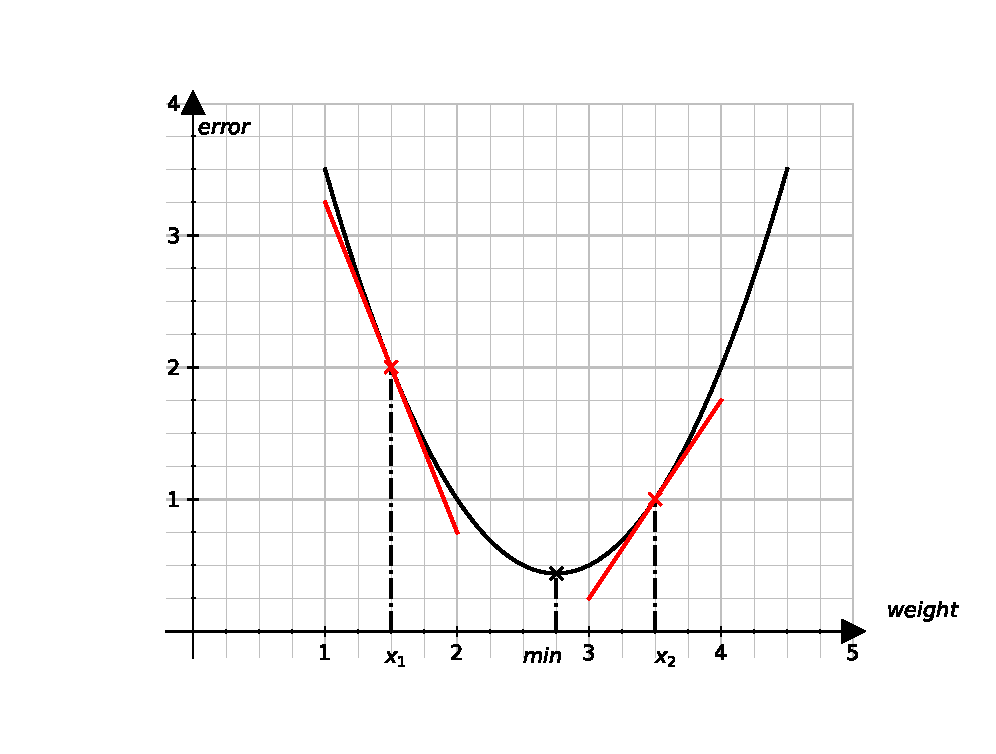
\includegraphics[scale=0.75]{CHAPTER_2/c2_fig_network_error_python.eps}
  \caption{Network Error over different weight}
  \label{network_error_graph}
\end{figure}
\noindent Figure (\ref*{network_error_graph}) is a graphical representation of the network error function. Our goal is to reach the minimum of the function by adjusting the weight value.
\subsection*{Gradient Descent}
In order to reach the bottom of the function; we need to adjust the weight such that the derivative of the error function is 0. The approach of updating the weight based on the gradient of the error function is known as \textbf{gradient descent}. The derivative with respect to the weights of the network error (\refeq{network_error}) for a single input is given by
\begin{align}
  \frac{\partial e}{\partial w_{ij}} = (\widehat{y_i}-y_i)\frac{\partial \widehat{y_i}}{\partial w_{ij}}
  \label{derivative_network_error}
\end{align}
From figure (\refeq{network_error_graph}); we can observe that if the gradient is negative then we have underestimated the predicted value and need to increase the weight to reach the optimal value. On the other hand, if the gradient is positive then we have overestimated the predicted value and need to decrease the weight to reach the optimal value. The equation (\refeq{derivative_network_error}) provides us with the opposite direction and amount to adjust the weight. Hence, the update rule of the weights for gradient descent method is given by
\begin{align}
  w_{ij}^{t+1} = w_{ij}^{t} - \dfrac{de}{dw_{ij}}
\end{align}
In the gradient descent method, the network learns from the gradient of the error function and adjust the weights accordingly to reduce the error. However, the gradient alone can be quite large, causing oscillations as we go down the error function. This problem by introducing a \textbf{learning rate} $\alpha$ prior to adjusting the weight.
\subsubsection*{Learning Rate}
The learning rate is typically denoted by the Greek letter alpha $\alpha$. It helps the network to control the rate at which the weights are changing. Having a system with a high learning rate may lead to an oscillating network when trying to find the optimal weight and having a slow learning rate increases the number of iterations required when optimizing the network. The adjusted update rule of the weight is given by
\begin{align}
  w_{ij}^{t+1} = w_{ij}^{t} - \alpha\dfrac{\partial e}{\partial w_{ij}}
\end{align}
where $\alpha \in (0,1)$
\subsection*{Stochastic Gradient Descent}
The Stochastic Gradient Descent dates back to the Robbins-Monro algorithm from the 1950s and is still an important optimization algorithm \cite{Robbins1951}. Instead of adjusting the weight to the average loss function, we can approximate the gradient by only one random directional derivative of the error. Thus, the number of computation in the gradient descent method can be significantly reduced by a factor of $n$ (where $n$ is the number of direction). The stochastic gradient method (SGM) is given by 
\begin{align}
    \label{eq:SGM_def}
    w^{t+1} = w^{t} - \alpha_t {(\nabla e)}_i
\end{align}
where $\alpha_t$ is the learning rate at the $t^{th}$ iteration which may vary with iterations.\\
As we move closer to the bottom of the minimum of the function; the solution starts to oscillate since we are moving the weight in random directions. Thus, the learning rate should be reduced gradually as we iterate. Some commonly used reduction of learning rate is given by 
\begin{align}
    \label{eq: learning_rates}
        \eta(t) &= \eta_i \,\,\, \,\,\,\, \text{ if } t_i \leq t \leq t_{i+1} &\text{piecewise constant} \\
        \eta(t) &= \eta_0e^{-\lambda t} &\text{exponential decay} \\
        \eta(t) & = \eta_0 (\beta t + 1)^{-\alpha} &\text{polynomial decay}
\end{align}
where $\lambda$, $\beta$, and $\alpha$ are known as hyperparameter. \\
Training dataset can be very large in certain cases which leads to a greater cost of compute at each iteration for the gradient descent, so stochastic gradient descent is preferred in these cases.
\subsection*{Mini-Batch Stochastic Gradient Descent}
In order to make use of the features of both gradient descent and stochastic gradient descent; we introduce the mini-batch stochastic gradient descent. In this approach, instead of iterating in the direction of the full gradient or only in one direction of the full gradient, we split the dataset into small batches and compute the gradient of each batch. The formula of the stochastic gradient descent is given by 
\begin{align}
    \label{mb-sgd}
    \textbf{w}^{t+1} &= \textbf{w}^{t} - \eta_t \textbf{g}_t \\
    \nonumber
    \textbf{g}_t &= \nabla_{\mathcal{B}_t}e(\textbf{x},\textbf{w}) 
\end{align}
where $\mathcal{B}_t$ is a mini-batch of elements drawn uniformly at random from the training set (the expectation of the gradient remains unchanged). \\ Since we are using a mini-batch, the updates are closer to the full gradient but at a reduced cost.
\subsection*{Newton's Method}
For minimizing $f(x)$, $x \in \mathbb{R}$, we need to solve $g(x) = e^{'}(x)=0$. Newton's iteration is given by 
\begin{align}
  x_{n+1} &= x_{n} - \dfrac{g(x_{}n)}{g^{'}(x_n)} \\
          &= x_{n} - \dfrac{f^{'}(x_{}n)}{f^{''}(x_n)}
\end{align}
For multivariate functions we need to minimise $f(\mathbf{x})$ over $\mathbf{x} \in \mathbb{R}^n$, that it
\begin{align}
  \begin{matrix}
    \underset{\mathbf{x}\in\mathbb{R}^n}{min} f(\mathbf{x}), & \,\,\, \mathbf{x} =(x_1,x_2,\dots,x_n)^T \in \mathbb{R}^n
  \end{matrix} 
\end{align}
The Newton's iteration for multivariate function is given by
\begin{align}
  \mathbf{x_{n+1}} = \mathbf{x_{n}} - H(\mathbf{x_n})^{-1}\nabla f(\mathbf{x_n})
\end{align}
where $H(\mathbf{x_n})$ is the Hessian matrix of $f(\mathbf{x})$.\\
\noindent We can observe from (\refeq{eq:Hessian_matrix}) that calculating the inverse of the Hessian matrix can be computationally very expensive for higher dimensions. Replacing $H(\mathbf{x_n})^{-1}$ by $\alpha \mathcal{I}$ where $\mathcal{I}$ is the identity matrix; we get the \textbf{method of steepest descent} given by
\begin{align}
  \mathbf{x_{n+1}} = \mathbf{x_{n}} - \alpha \textbf{I} \nabla f(\mathbf{x_n})
\end{align}
where $\alpha \in (0,1)$
\subsection*{Momentum}
%https://ui.adsabs.harvard.edu/abs/1986Natur.323..533R/abstract
%Documention on when momentum first appeared
\subsubsection*{Exponentially Weighted Moving Average}
The exponentially weighed moving average (EWMA), also known as exponential moving average (EMA), of a series of data points $S_t$ is given by 
\begin{align}
    \label{eq:ewma_def}
    \mu_t &= \beta \mu_{t-1} + (1-\beta)S_t \\
    \nonumber
    \mu_0 &= c
\end{align}
where $c \in \mathbb{R}$ and $\beta \in (0,1)$ is known as the smoothing constant. $\beta$ represents the weightage that is going to be assigned to the past values. The average number of previous reading is approximately given by $n={(1-\beta)}^{-1}$. The higher the value of $\beta$ the greater the number of points we average over.
\subsubsection*{SGD with Momentum}
The momentum method was mentioned in Rumelhart, Hinton and Williams' paper on back-propagation learning in 1986 \cite{Rumelhart:1986aa}.  From the SGD, it was observed that the weight update can be very noisy. In order to smoothen the search direction in the SGD, an exponentially moving average is implemented on the gradient. The SGD with momentum can be written in the form
\begin{align}
    \label{eq: SGF_with_momentum}
    \textbf{w}^{t+1} &= \textbf{w}^{t} - \eta \boldsymbol{\mu}^t
    \intertext{where the exponential moving average of the gradient is given by}
    \nonumber
    \boldsymbol{\mu}^{t} &= \beta \boldsymbol{\mu}^{t-1} + (1-\beta)\nabla(e)^t \\
    \nonumber
    \boldsymbol{\mu}_0 &= \textbf{c}
\end{align}
\subsection*{RMSProp}
%https://www.scirp.org/(S(czeh2tfqyw2orz553k1w0r45))/reference/ReferencesPapers.aspx?ReferenceID=1911091
Proposed by Geoffrey Hinton in lecture 6 of the online course "Neural Network for Machine Learning" \cite{Hinton2012}, the Root Mean Square Propagation (RMSProp) algorithm alleviates undesirable fluctuations when adjusting the weight during optimization. RMSProp is an adaptive learning rate. The idea is to reduce the step size at very large gradient to avoid fluctuations and increase the step size at smaller gradient to move steadily in the correct direction of the optimal solution; hence an adaptive learning rate at each iteration. The equations for the RMSProp is given by 
\begin{align}
    \nonumber
    \label{eq:RMSProp_def}
    {S}^t_i &= \gamma {S}^{t-1}_i + (1-\gamma)(\nabla e^t)_i^2 \\
    {w}^{t+1}_i &= {w}^t_i - \dfrac{\eta}{\sqrt{S^t_i} + \epsilon}(\nabla e^t)_i
\end{align}
where $\epsilon \approx 10^{-6}$ to ensure that we avoid dividing by zero during iterations.
\subsection*{Adam}
%https://arxiv.org/abs/1412.6980
The Adam algorithm (Adaptive Moment Estimation algorithm) is a robust update rule for the weight optimization \cite{Kingma2014}. The algorithm combines the benefits of momentum (\refeq{eq: SGF_with_momentum}) and RMSProp (\refeq{eq:RMSProp_def}). Adam is the most popular generalized algorithm performs very well in many cases. It is considered as a state-of-the-art algorithm for deep neural network optimization. The set of equations for the Adam algorithm is given by
\begin{align}
    \nonumber
    \mu^{(t)}_i &= \beta_1 {\mu}^{(t-1)}_i + (1-\beta_1)\nabla(e^{(t)})_i &\text{Momentum} \\
    \nonumber
    {S}^{(t)}_i &= \beta_2 {S}^{(t-1)}_i + (1-\beta_2)(\nabla e^{(t)})_i^2 &\text{RMSProp}    
\end{align}
To prevent $S^t$ and $\mu^t$ from becoming zero during the initial steps, a bias correction is introduced, such that
\begin{align*}
    \hat{\mu^{(t)}} = \dfrac{\mu^{t}}{1-\beta_1^t} & & \hat{S^{(t)}} = \dfrac{S^t}{1-\beta_2^t}
\end{align*}
Finally, the update rule is given by
\begin{align}
    \label{eq:Adam_def}
    {w}^{(t+1)}_i &= {w}^{(t)}_i - \dfrac{\eta}{\sqrt{S^t_i} + \epsilon}\mu_i
\end{align}
The parameters $\beta_1$, $\beta_2$ and $\epsilon$ are knows are the hyperparameters of the Adam algorithm. A common set of values that works well in literature are $\beta_1 = 0.9$, $\beta_2 = 0.9999$ and $\epsilon = 10^{-8}$ \cite{Kingma2014}.
%https://arxiv.org/pdf/1412.6980.pdf
\section{Backpropagation using Adam}
The Adam algorithm for optimization can be introduced in the weight update when training deep neural network. The problem of finding the right set of weights and biases for a deep neural network can be reduced to an optimization problem same as we defined in (\refeq{network_error}). After finding the gradients through the backpropagation algorithm, the set of updates proposed in the Adam algorithm are used to update the weights and biases in the neural network.
\begin{algorithm}[H]
  \caption{Backpropagation using Adam optimization with $n$ total number of inputs for $N$ epochs}\label{alg:back_propagation_adam_algo}
  \begin{algorithmic}[1]
  \State{\textbf{Start}}
  \For{$t = 1,2, \dots, N$}
  \For{$s = 1,2, \dots, n$}
  \State Compute the activation layer $a^{(1)}$ using $n$ input values in a batch
  \State $a^{(1)} = \sigma(w^{(1)}x + b^{(1)} )$
  \State Feed forward the $n$ input to the next layers
  \For{$l = 2,3,\dots,L$}
    \State{$z^{(l)} = w^{(l)}a^{(l-1)}+b^{(l)}$}
    \State $a^{(l)} = \sigma(z^{(l)})$
  \EndFor  
\EndFor
  \State Compute the average cost function, $C$, at the output layer $L$
  \State $c^{(t)} = \dfrac{1}{2n}\sum^{n}_s (\widehat{y_s}-y_s)^2$
  \State Compute the rate of change of the cost function $w.r.t$ to $z^{(L)}$
  \State $\delta^{(L)} = \nabla_{a^{(L)}}C \odot \sigma^{'}(z^{(L)})$
  \For{$l = L-1, L-2, \dots, 2$} 
    \State Computing the gradients
    \State $\delta^{(l)} = (w^{(l+1)})^T\sigma^{(l+1)} \odot \sigma^{'}(z^{(l)})$
    \State $\nabla_{b^{(l)}} C = \delta^{(l)}$
    \State $\nabla_{w^{(l)}} C = \delta^{(l)}a^{(l-1)}$\\
    \State Bias update
    \State $\mu^{(t)}_i = \beta_1 {\mu}^{(t-1)}_i + (1-\beta_1)\delta^{(l)}_i$
    \State ${S}^{(t)}_i = \beta_2 {S}^{(t-1)}_i + (1-\beta_2)(\delta^{(l)}_i)^2$
    \State $\hat{\mu^{(t)}} = \dfrac{\mu^{t}}{1-\beta_1^t}$
    \State $ \hat{S^{(t)}} = \dfrac{S^t}{1-\beta_2^t}$
    \State ${b}^{(t+1)}_i = {b}^{(t)}_i - \dfrac{\eta}{\sqrt{S^t_i} + \epsilon}\mu_i$\\
    \State Weight update
    \State $\mu^{(t)}_i = \beta_1 {\mu}^{(t-1)}_i + (1-\beta_1)\delta^{(l)}a^{(l-1)}_i$
    \State ${S}^{(t)}_i = \beta_2 {S}^{(t-1)}_i + (1-\beta_2)(\delta^{(l)}a^{(l-1)}_i)^2$
    \State $\hat{\mu^{(t)}} = \dfrac{\mu^{t}}{1-\beta_1^t}$
    \State $\hat{S^{(t)}} = \dfrac{S^t}{1-\beta_2^t}$
    \State ${w}^{(t+1)}_{ij} = {w}^{(t)}_{ij} - \dfrac{\eta}{\sqrt{S^t_i} + \epsilon}\mu_i$
  \EndFor
\EndFor
\end{algorithmic}
\end{algorithm}
\chapter{Sentiment Analysis}
People's opinions, feelings and sentiments towards entities such products, services, other people, events, news, issues, topics, etc. can be in very large volume, complex and difficult to be understood and processed by machines and computers. Thus, sentiment analysis, also known as opinion mining, started to popularised along the rise of social media when large amount of digital text data were suddenly available for mining. Natural language processing (NLP) helps computers process and understand human based language to perform repetitive task. Sentiment analysis is a niche of NLP. It aims at quantifying the positivity, negativity and/or neutrality of implied or expressed in a given text.

Social media have been providing large platforms for people to share their opinion freely and expressed their views on any subject across various geographical and spatial  boundaries. They have also allowed people to connect, influence and be influenced by such opinions and views. These interactions have been studied in the 1940s and 1950s among people in organizations by management science researchers. Since 2002, with social media, those studies have been performed at grand scales with the abundance of data. Thus, advanced sentiment analysis research have been performed in field political science, economics, finance and management science as they are heavily dependent on public opinions. 

Asur and Huberman (2010) (ADD REF) attempted to solve the revenue prediction problem using both the tweet volume and the tweet sentiment. Same kind of data along with polling results were also used, in Bermingham and Smeaton (2011) (ADD REF), to train a linear regression model to predict election results. Zhang et al. (2010) (ADD REF) leveraged sentiments on Twitter to help predict the movement of stock market indices such as Dow Jones, S\&P500 and NASDAQ. It was shown that large negative emotions and opinions caused Dow to go down the next day and lower negative emotions cause Dow to go up on the next day. Bar-Haim et al. (2011) (ADD REF) on one hand leverage sentiments on Twitter but on the other did not treat all Twitter authors equally. Only expert investors were used as features in training stock price movement predictors. Undeniably, modern social media (started early 2000s) have grown into a major influencer of human opinion and sentiments.

%VADER?
%LSTM
%BERT
%RoBERTa
\chapter{Tweet Data}
\section{Tweets}
\subsection{Tweepy}
\subsubsection{Scrapping using Tweepy}
\subsubsection{Cleaning using RegEx}
\section{Tweet Count}
\section{Tweet Search Volume Index (SVI)}
\section{Feature Engineering}
\chapter{Conclusion and Future Works}

This study investigated how we can leverage deep learning models and sentiment analysis on tweets to predict the value of Bitcoin in the next hour. 

We reviewed the basics and derived the backpropagation algorithm of feed-forward neural networks. An application of the backpropagation algorithm for feed-forward neural networks was derived. Moreover, we investigated the literature and defined different architectures of sequential neural networks used in problems involving sequential data. The literature on optimization algorithms was also reviewed. We looked at the application of the Adam optimizer in the backpropagation algorithm, the current state-of-the-art algorithm for the optimization problem. We also briefly examined sentiment analysis literature using traditional methods and the latest deep learning models involving transformers for natural language processing, roBERTa (Robustly Optimized BERT Pre-training Approach).

Finally, we defined and coded a whole pipeline from scrapping data to predicting the value of Bitcoin in the next hour using the LSTM NN model. Scrapping, cleaning and feature engineering raw data is tedious. The RMSE for the training and testing on the whole dataset were \$303.96 and \$325.96, respectively. We saw a slight decrease in performance when using only the influencers' data which might be due to the naive way we used to identify influencers: by only considering their number of followers. Furthermore, deep learning models are not easily interpretable due to their BlackBox-like architecture. It did involve a significant amount of trial.

As a continuity to this work, it would be interesting to compare our model to traditional statistical models. Additionally, we could investigate the features to be added in the LSTM NN model and/or identify the dominant features to reduce our dataset (potentially decreasing training time).
\bibliography{REFERENCES}
%\chapter{Placeholder - to be deleted}
\section{Linear Algebra}
We introduce briefly the realm of linear algebra to get a better understanding of more complex concepts in neural networks. The focus is set on mainly the properties useful in deep learning. \\
Linear algebra is the study of linear equations of the form:
\begin{equation}
    x_1a_1 + \dots + x_na_n = b
\end{equation}
or as a linear map defined by the following:
\begin{equation}
    (x_1, \dots, x_n) \mapsto (a_1 x_1 + \dots + a_n x_n) \label{eq:2.11}
\end{equation}
and their representation, manipulation and operation using vectors and matrices within a set of predefined axioms. 
\subsection{Vectors}
A vector is quantity that has both a magnitude and direction. It can be represented by an ordered set of numbers or graphically using an arrow.
Consider the vector \textbf{u} in $\mathbb{R}^2$ given by:
\begin{align}
    \textbf{u} &= \begin{bmatrix}
           u_1 \\
           u_2 \\
         \end{bmatrix}
  \end{align}
The vector can be expressed graphically as shown below.
\begin{center}
    *Image Placeholder vector in $R^2$*    
\end{center}

\noindent The length of the arrow is an indication of the magnitude of a vector and its orientation given by the direction in which the arrow is pointing. The magnitude of the above vector can be computed as such:
\begin{align}
    ||\textbf{u}|| = \sqrt{u_1^2+u_2^2}
\end{align}

\noindent The direction of the vector with respect to the $x$-axis is given by: 
\begin{align}
    \theta = \tan^{-1}\left(\dfrac{u_2}{u_1}\right)
\end{align}
A vector space is a set of vectors which satisfy the following axioms:
\begin{center}
    *Placeholder - Table of Axioms for Vector Space*    
\end{center}
\noindent\textbf{Geometry representation of addition and subtraction of vectors in $\mathbb{R}^2$}
Vector addition and subtraction is performed componentwise along each element of two vectors. Consider the two vectors $\textbf{a}$ and $\textbf{b}$ where:
\begin{align}
    \textbf{u} = \begin{bmatrix}
        u_1 \\
        u_2 \\
      \end{bmatrix},
      \textbf{v} = \begin{bmatrix}
        v_1 \\
        v_2 \\
      \end{bmatrix}
\end{align}
\noindent\textbf{Addition} \\
The addition of vector $\textbf{u}$ and $\textbf{v}$ is given by:
\begin{align}
    \textbf{u} + \textbf{v} =
      \begin{bmatrix}
        u_1 + v_1 \\
        u_2 + v_2 \\
      \end{bmatrix}
      \label{eq:addition_vectors}
\end{align}
The geometrical effect of adding $\textbf{u}$ and $\textbf{v}$ together is shown below.
\begin{center}
    *Image Placeholder vector addition in $R^2$*    
\end{center}
We can observe from (image ref) above that adding $\textbf{u}$ to $\textbf{v}$ has the effect of rotating $\textbf{u}$ towards $\textbf{v}$.

\noindent\textbf{Subtraction} \\
The subtraction of vector $\textbf{v}$ from $\textbf{u}$ is given by:
\begin{align}
    \textbf{u} - \textbf{v} =
      \begin{bmatrix}
        u_1 - v_1 \\
        u_2 - v_2 \\
      \end{bmatrix}
      \label{eq:subtraction_vectors}
\end{align}
\begin{center}
    *Image Placeholder vector subtraction in $R^2$*    
\end{center}
We can observe from (image ref) above that subtracting $\textbf{v}$ from $\textbf{u}$ has the effect of rotating $\textbf{u}$ in the opposite direction of $\textbf{v}$.\\
\vspace{1mm}
\noindent The effect of rotating two vectors though addition and subtraction are useful properties utilized in deep learning.
\subsubsection{Inner Product}
\noindent The inner product or dot product of: 
\begin{align}
    \textbf{u} = \begin{bmatrix}
        u_1 \\
        u_2 \\
      \end{bmatrix},
      \textbf{v} = \begin{bmatrix}
        v_1 \\
        v_2 \\
      \end{bmatrix}
\end{align}
is given by $\textbf{u}.\textbf{v}$
\begin{align}
  \textbf{u.v} &= u_1 v_1 + u_2 v_2 \\
  &= ||\textbf{u}|| \, ||\textbf{v}||\cos \theta
  \label{eq:cosine_rule_dot_product}
\end{align}
where $\theta$ is the angle between vectors \textbf{u} and \textbf{v}.
\begin{center}
  *Image Placeholder inner product in $R^2$*    
\end{center}
The dot product of $\textbf{u.v}$ equals \textbf{v.u}. The order does not make a difference.
\subsection{Matrices}
\noindent A matrix is an $m \times n$ array of numbers, where $m$ is the number of rows and $n$ is the number of columns; the matrix is said to be of dimension $(m \times n)$.
\begin{align}
  \textbf{A} = 
  \begin{bmatrix}
    a_{11} & a_{12} & \dots & a_{1n} \\
    a_{21} & a_{22} & \dots & a_{2n} \\
    \vdots & \vdots & \ddots & \vdots \\
    a_{m1} & a_{m_2} & \dots & a_{mn}
  \end{bmatrix}
\end{align}
Similar to vectors, there are a couple of matrix operations that can be done under certain condition. \\
\noindent \textbf{Matrix Operations} \\ 
\noindent \textbf{Matrix Addition} \\
The sum of two matrices $\textbf{A}$ and $\textbf{B}$ is given by the element wise sum of the elements provided that they both have the same dimension. 
\\ Consider two matrices \textbf{A} and \textbf{B}:
\begin{align}
  \textbf{A} =
  \begin{bmatrix}
    a_{11} & a_{12} \\
    a_{21} & a_{22}
  \end{bmatrix} \, \, \, 
  \textbf{B} =
  \begin{bmatrix}
    b_{11} & b_{12} \\
    b_{21} & b_{22}
  \end{bmatrix}
\end{align}
 the sum \textbf{A + B} is given by
\begin{align}
  \textbf{A} + \textbf{B} = \begin{bmatrix}
    a_{11} + b_{11} & a_{12} + b_{12} \\
    a_{21} + b_{21} & a_{22} + b_{22}
  \end{bmatrix}
\end{align}\\
\noindent \textbf{Scalar Matrix Multiplication} \\
The product $\alpha\textbf{A}$, where $\alpha \in \mathbb{R}$ and $\textbf{A}$ is a matrix, is calculated by multiplying every entry of $\textbf{A}$ by $\alpha$. \\
Consider  a matrix \textbf{A} and constant $\alpha$:
\begin{align}
  \begin{bmatrix}
    a_{11} & a_{12} \\
    a_{21} & a_{22}
  \end{bmatrix}
\end{align}
the scalar multiplication $\alpha \textbf{A}$ is given by
\begin{align}
  \alpha \textbf{A} = 
  \alpha \begin{bmatrix}
    a_{11} & a_{12} \\
    a_{21} & a_{22}
  \end{bmatrix}
  = \begin{bmatrix}
    \alpha a_{11} & \alpha a_{12} \\
    \alpha a_{21} & \alpha a_{22}
  \end{bmatrix}
\end{align} \\
\noindent \textbf{Matrix Transpose} \\
\noindent The transpose of a $(m \times n)$ matrix $\textbf{A}$ is calculated by swapping the rows into columns or the columns into rows. This operation result in a $(n \times m)$ denoted as $\textbf{A}^T$. \\
Consider  a matrix \textbf{A}, the transpose is given by $\textbf{A}^T$:
\begin{align}
  \textbf{A} = \begin{bmatrix}
    a_{11} & a_{12} \\
    a_{21} & a_{22}
  \end{bmatrix} \, \, \, 
  \textbf{A}^T = \begin{bmatrix}
    a_{11} & a_{21} \\
    a_{12} & a_{22}
  \end{bmatrix}
\end{align}
\noindent \textbf{Matrix Multiplication} \\
The multiplication operation between two matrices is only defined is the number of columns of the left matrix is the same as the number of rows in the right matrix. If \textbf{A} is a $(m \times n)$ matrix and \textbf{B} is a $(n \times p)$ matrix, then their product \textbf{AB} is the $(m \times n)$ matrix whose entries are given by inner product of the corresponding row of \textbf{A} and the corresponding column of \textbf{B}.\\
Consider two matrices \textbf{A} and \textbf{B}:
\begin{align}
  \textbf{A} =
  \begin{bmatrix}
    a_{11} & a_{12} & a_{13} \\
    a_{21} & a_{22} & a_{23}
  \end{bmatrix} \, \, \, 
  \textbf{B} =
  \begin{bmatrix}
    b_{11} & b_{12} \\
    b_{21} & b_{22} \\
    b_{31} & b_{32}
  \end{bmatrix}
\end{align}
 the matrix multiplication is given by \textbf{AB}
\begin{align}
  \textbf{A}\textbf{B} &= \begin{bmatrix}
    a_{11} & a_{12} & a_{13} \\
    a_{21} & a_{22} & a_{23}
  \end{bmatrix} \begin{bmatrix}
    b_{11} & b_{12} \\
    b_{21} & b_{22} \\
    b_{31} & b_{32}
  \end{bmatrix} \\
  &= \begin{bmatrix}
    a_{11}b_{11} + a_{12}b_{21} + a_{13}b_{31} &  a_{11}b_{12} + a_{12}b_{22} + a_{13}b_{32} \\
    a_{21}b_{11} + a_{22}b_{21} + a_{23}b_{31} &  a_{21}b_{12} + a_{22}b_{22} + a_{23}b_{32}
  \end{bmatrix}
\end{align}
\subsubsection{Outer Product}
\noindent The outer product of two vectors $\textbf{u}$ and $\textbf{v}$: 
\begin{align}
    \textbf{u} = \begin{bmatrix}
        u_1 \\
        u_2 \\
      \end{bmatrix} \, \, \, 
      \textbf{v} = \begin{bmatrix}
        v_1 \\
        v_2 \\
      \end{bmatrix}
\end{align}
is given by $\textbf{u}\otimes\textbf{v}$
\begin{align}
  \textbf{u}\otimes\textbf{v} = \begin{bmatrix}
    u_1v_1 & u_1v_2 \\
    u_2v_1 & u_2v_2
  \end{bmatrix}
\end{align}
The outer product of $\textbf{u}\otimes\textbf{v}$ is not equal to $\textbf{v}\otimes\textbf{u}$; the order does matter. However, the transpose of latter outer product are the same:
\begin{align}
  \textbf{u}\otimes\textbf{v} = (\textbf{v}\otimes\textbf{u})^T 
\end{align}
\chapter{test}
\end{document}